\section{Inference Methodology}

%For the SEI:

%Census data + geolocalization + ARPU + cellphone payments (recharges)  --> SEI estimation for geolocalized users. 

%Second, we extended our predictions taking advantage of graph structure and socioeconomic homophily. To this end, we considered a bayesian  

%\sout{As part of the dataset from the bank \( B \), we have the monthly salaries of most bank users \( B_{S_0} \cdots B_{S_t} \) for a period \( t \) larger than \( M \). We considered the average of \( B_{S_i} \) for a period of \( 6 \) moths to generate \( B_S \)}

%\sout{To infer the monthly salary of the users we take the average of \( B_{S_i} \) for a period of \( 6 \) moths to generate \( B_S \), and we compare them with other users' salaries by using the link correlations in \( G_N \).}

The main contribution of this work is the estimation of the income of the telco users for which we lack banking data but have bank clients in their neighborhood of network graph. To show the feasibility of this task we first show the existence of a strong income homophily in the telco graph as is evidenced in figure \ref{homophily_heatmap}.

For each pair \( \left< o, d \right> \in \mathlarger{G} \) we define \( X \) as the set of incomes for callers and \( Y \) as the set of incomes for callees. According to what we can observe in Figure \ref{homophily_heatmap}, \( X \) and \( Y \) should be significantly correlated. Given the broad non gaussian distribution of the income's values, we choose to use a rank based measure of correlation, namely the \textbf{Spearman's rank correlation} to test the statistical dependence of sets \( X \) and \( Y \) using the following formula: 

\[
r_s = \mathlarger{\rho}_{\operatorname{rank}(X) \operatorname{rank}(Y)} = \frac{\operatorname{cov}(\operatorname{rank}(x), \operatorname{rank}(y))}{\sigma_{\operatorname{rank}(X)} \sigma_{\operatorname{rank}(Y)}}
\]

If we compare our data with a randomized null hypothesis, where links between users are selected randomly disregarding income data, this coefficient gives us a correlation coefficient of $r_s = \mathbf{0.474} $ with a P-value of $ \mathbf{P < 10^{-6}} $. This is significant enough to show that there is an important amount of homophily between users' incomes in our data.

We can take advantage of this homophily to propagate income information to the rest of our graph $ \mathlarger{P} $, where we don't know the income of all of the users.

\begin{figure}[h]
\begin{center}
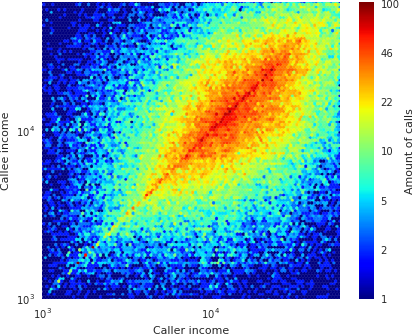
\includegraphics[width=1\columnwidth]{figures/Homophily_income_origin_target_1/Homophily_income_origin_target_1.png}
\caption{ \protectReplace this text with your caption}
\label{homophily_heatmap}
\end{center}
\end{figure}

\subsection{Prediction algorithm}

Instead of attempting to predict the exact value of a user's income we partition the set of possible income values into five groups that were deemed usefull for the Bank: $[1000,2500),[2500,7500),[7500,20000),[20000,50000),[50000,+50000)$, values are given in Mexican pesos.  

To define the result of the prediction in exact terms, we discretize the income distribution into 5 equally sized groups, $ H_1, \ldots, H_5 $ of increasing wealth, where

\[
\left( \forall g \in H_i, g' \in H_{i + 1} \right) g_s < g'_s
\]

For each user $ g \in \mathlarger{G} $ we define its call distribution to other income categories as $ g_{\alpha_1} \ldots g_{\alpha_5} $, and we use those distrubutions as the parametrization of a \textbf{Dirichlet Distribution}. We interpret the sample space of $ D(\alpha_p) $ as a discrete probability distribution by considering our initial assumption of data homophily, where we expect users belonging to a certain category to have calls concentrated to other users of that particular one.

Each user has a caller category probability density function of the form

\[
f \left( x_1, \ldots, x_5; \alpha_1, \ldots, \alpha_5 \right) = \frac{1}{\Beta \left( \alpha \right)} \prod^5_{i = 1} x_i^{\alpha_i - 1}
\]

Where $ \Beta $ represents the Beta function,

\[
\Beta \left( \alpha_1, \ldots, \alpha_k \right) = \frac{\prod^k_{i = 1} \Gamma \! \left( \alpha_i \right)}{\Gamma \! \left( \sum^k_{i = 1} \alpha_i \right) }
\]

For all the other users in the telco $ q \in Q = (N \setminus G) $, we can use this distribution to infer the probabilities of being part of each group $ H_1, \ldots, H_5 $, and this way approximate the economic status.
